\chapter*{Conclusion}
\addcontentsline{toc}{chapter}{Conclusion} % To add to TOC

\initial{I}t is now time to conclude this document, whose purpose was twofold:
exhibit clear theoretical properties of analogical classifiers, and apply
analogical inference to the field of recommender systems. Let us first recap
our main results and contributions (we will not necessarily follow the order of
the chapters here).

\paragraph{Contributions\\}

The first chapter was dedicated to give the necessary background on existing
models of analogical reasoning,  with a strong emphasis on models that allowed
to build computer programs. In the second chapter, we thoroughly described
various definitions of analogical proportions in different settings, with a
particular focus on the arithmetic and Boolean proportions. We have tried to
provide the reader with different geometrical insights on these proportions,
which were hopefully useful to gain a better intuition.
Finally, we considered a toy classification problem in a Boolean setting that
allowed us to introduce the analogical equation solving process and most
importantly, our analogical inference principle. This principle states that if
we have $a:b::c:d$, then we should also have $f(a) : f(b) :: f(c):f(d)$, where
$f(x)$ is the label of $x$, or any characteristic of interest.  When $f(d)$ is
unknown, it can be \textbf{inferred} from the values of $f(a)$, $f(b)$ and
$f(c)$, allowing us to apply this form of analogical reasoning to
classification tasks, or more general problems such as that of rating
prediction for recommendation tasks.\\

Analogical recommendation was addressed in Chapters
\ref{CHAP:background_reco_systems} and \ref{CHAP:analogical_recommendation}.
Chapter \ref{CHAP:background_reco_systems} was a background chapter, where we
clearly defined the problem we planned to address, and described two popular
collaborative filtering families (neighborhood methods and
matrix-factorization techniques) that will be compared to our custom algorithms
in the experiments.

We then developed in Chapter \ref{CHAP:analogical_recommendation} an algorithm
for rating prediction \cite{HugPraRicISMIS15}, on the basis that if four users
are in proportion (i.e. their respective ratings are in arithmetic proportion),
then it should also be the case for any item that one of the four users has not
rated. This approach is directly inspired from past works on analogical
classification. The experiments showed that this algorithm offers reasonable
performance compared to neighborhood techniques, but its cubic complexity makes
it simply impossible to use in real-world scenarios, due to enormous
computation time.

This led us to consider another kind of analogical recommendation, that does
not rely on the search of $3$-tuples of users. This ``clone''-based view
\cite{HugPraRicSerFuzzIEEE16} is motivated by the fact that some users may
have different interpretations of the rating scale that is used. Our results
show that the concept of ``clone'' is extremely relevant, but it must be noted
that this kind of bias in the user ratings had already been addressed in
previous works.

Finally, we provided an algorithm for the mining of analogical proportions in
incomplete databases \cite{HugPraRicSerLFA16}, strongly inspired from the
mining of association rules. We used this algorithm to extract analogical
proportions between items in a rating database, which actually corresponds to
the database that we had been using for our recommendation experiments. Our
results showed that the analogies we found were in fact rather
uninteresting, in that they related four items that were either equally
appreciated, or equally disliked. There was no discrepancy in the ratings. In
a way, this fact can retrospectively explain the modest results of our first
analogical recommendation algorithm, and its performances that were close to
those of neighborhood methods.\\

In Chapter \ref{CHAP:functional_definition}, we described our contributions to
the field of analogical classification \cite{HugPraRicSerECAI16}. Our first key
contribution was to provide a unifying functional definition of analogical
classifiers, which were yet only known from their algorithmic descriptions.
From this definition, we were able to derive various theoretical properties. In
particular, we showed that the VC-dimension of analogical classifiers is
infinite, and that their error rate is closely related to that of the $k$-NN
algorithms, as can be seen on the analytical formula that we derived. In fact,
our functional definition establishes clear links between analogical
classification and nearest-neighbors classification. We have showed indeed that
analogical classification can be viewed as a two-steps procedure: first the
training set is extended by analogy, where new examples are generated and
assigned a potentially noisy label called the analogical label. Then, using
this extended training set, all the remaining elements can be labeled using the
classical $k$-NN procedure. This new point of view is quite interesting,
because it clearly binds together the two processes triggered by analogical
proportions (inference and creativity) as the two sides of the same coin.

In Chapter \ref{CHAP:analogy_preserving_functions}, we investigated a question
that naturally followed from the results of Chapter
\ref{CHAP:functional_definition}: how can we ensure that the analogical
extension is completely error-free? In other words, is there a criterion that
tells us that the new examples that are generated are associated to the correct
label? We have been able to answer this question in a Boolean setting: the
analogical extension is perfectly sound if and (only if) the Boolean function
$f$ underlying the label is an affine function. This strong result
\cite{CouHugPraRicIJCAI17} is reminiscent of that of Davies and Russel (see
Section \ref{SEC:Davies_and_Russel}), who provided a side condition that
allowed to safely use an analogical inference principle. Their analogical
inference principle was actually quite different from ours (although we could claim
that ours is a particular case of theirs), but the two approaches can be
considered similar from a general point of view. We extended our results to the
real setting and in the case where attributes are nominally-valuated. These
results open the door to various speculative research topics, that we will now
explore.

\paragraph{Future work\\}

In Section \ref{SEC:approximate_ap_functions}, we presented the concept of
approximate AP functions. Indeed in practice, there is no way
to know for sure if the function $f$ that we want to learn is completely
affine. So a clear topic of interest is to obtain statistical guarantees about
the quality of the analogical extension, depending on how far the function $f$
is from the set of affine functions. As previously mentioned, a result of the
following form would be extremely interesting:
$$P(\omegasf \geq \eta) > 1 - \delta,$$
where $\eta \in [0, 1]$ and $\delta \in [0, \frac{1}{2}]$ are functions
depending on $\epsilon$ and $\mid S \mid$. The value $\epsilon$ tells us that
$f$ is $\epsilon$-close from the set of affine functions.  We are currently
investigating a somewhat simpler question:
$$P(\omegasf < 1) < \delta,$$
where $\delta$ is still a function of $\epsilon$. In other words, we want to
have an upper bound of the probability of the event ``\textit{$\esfs$ is
unsound}''.\\

We have also seen during our experimentations that even though some functions are
highly not AP, the quality of the analogical extension may still be very high.
This is because of the majority-vote procedure that is applied when we compute
the analogical label of the elements. This aspect has been left out of the
discussion so far, but it is clear that it is a decisive step of our inference
process, and it has to be thoroughly studied to fully understand the analogical
classification process. We may for example suppose that some $3$-tuples should
be given a higher weight in the aggregation, on the basis of some particular
static criterion that still needs to be identified.\\

Another track of research can be motivated by looking at Figure
\ref{FIG:piecewise_affine}.
\begin{figure}[!h]
\centering
  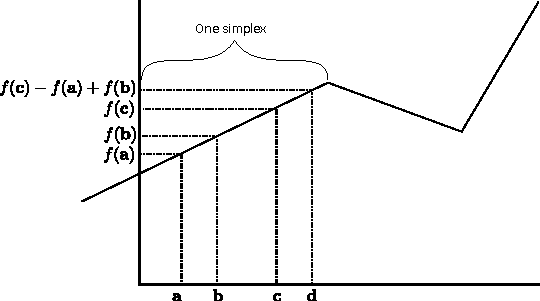
\includegraphics[width=3in]{figures/piecewise_affine.pdf}
  \caption{A real function $f$ that is piecewise affine.}
\label{FIG:piecewise_affine}
\end{figure}
The function $f$ is not affine, but is instead \textbf{piecewise affine}. We
know from our results that for any elements $\mathbf{a}, \mathbf{b},
\mathbf{c}, \mathbf{d} \in X^m$ that are on the same simplex (a simplex is here
defined as a subset of $X^m$ where $f$ is affine), then we can correctly
predict the value of $f(\mathbf{d})$ from those of $f(\mathbf{a}),
f(\mathbf{b}), f(\mathbf{c})$. Well in $\mathbb{R}^m$ this result is not really
useful, but we can actually show that every Boolean function is piecewise
affine! So theoretically, if we can identify all the simplices, this means that
we should be able to produce a sound extension in any case, for any function
$f$, and for any training set. At this point, only preliminary experiments
have been carried out, and a more thorough investigation deserves to be
addressed.\\

Finally, we will close this discussion by mentioning the elephant in the room
that we have so far ignored: transfer learning. Transfer learning is a current
trend in the machine learning community, whose purpose is to use the knowledge
of a source problem $S$, to apply it to a less known target problem $T$.
Undoubtedly, transferring knowledge is the essence of analogy, and techniques
in transfer learning usually involve statistical tools (see e.g.
\cite{PanYanTKDE10} for a survey). The use of analogical proportions for such
purposes is still entirely to be explored.
